\subsection{Esercizio 6}
Eseguendo lo script es6.m si ottengono i risultati contenuti nella tabella \ref{tab::1}
e nella figura \ref{fig::es6}. Come si può notare, il metodo di newton e il metodo delle secanti
convergono molto più rapidamente del metodo di bisezione e del metodo delle corde. 
\begin{table}[h]
\begin{tabular}{|l l l l l|}
        \hline
        Metodo & tolleranza$=10^{-3}$  & tolleranza$=10^{-6}$ & tolleranza$=10^{-9}$ & tolleranza$=10^{-12}$ \\
        \hline
        bisezione & 0.739257812500000 &  0.739085197448730  & 0.739085133187473 &  0.739085133215667\\
        newton   &  0.739085133385284 &  0.739085133215161  & 0.739085133215161 & 0.739085133215161 \\
        corde    &  0.739567202212256  & 0.739084549575213 & 0.739085132739254 & 0.739085133215737 \\
        secanti  &  0.739085133215001  & 0.739085133215161  &  0.739085133215161  &  0.739085133215161 \\
        \hline
\end{tabular}
\caption{valori approssimati}
\label{tab::2}     
\end{table}
\begin{figure}[h!]
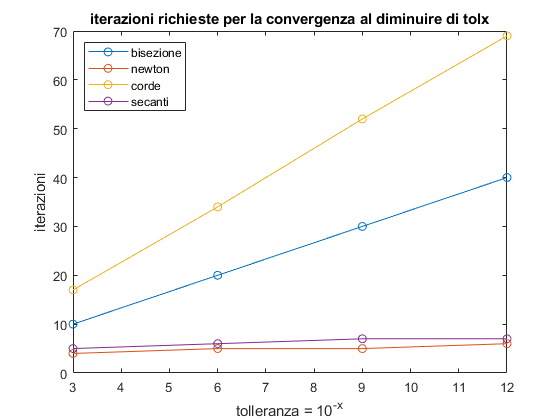
\includegraphics[scale=0.65]{capitolo2/iter.png}
\caption{iterazioni richieste}
\label{fig::es6}
\end{figure}
\


